\documentclass[letterpaper,12pt]{article}
\usepackage{fullpage}
\usepackage[pdftex]{graphicx}
\usepackage{amsmath}
%\usepackage{simplemargins}
%\setallmargins{0.5in}

\bibliographystyle{unsrt}


\title{Time Evolution of Gaussian Wave Packet by Each eigen State of 1 D Harmonic Oscillator}
\author{Susan Sapkota}
\date{\today}

\begin{document}
\maketitle
\begin{abstract}
Given Gaussian Wave Packet centered at the origin and other than origin,we want to findout contribution of each eigen state of the 1 D harmonic oscillator and oscilliate throughout time. for the energy eigen function, we findout solution to  Schrodinger equation of harmonic oscillator  using Hermite polynomial. Here we findout projection of wave packet onto each eigen states which is probability coefficient of each eigen function.Then we used time dependent solution for Schrodinger equation sum over each eigen state and evolve in time.
\end{abstract}
\begin{figure}
  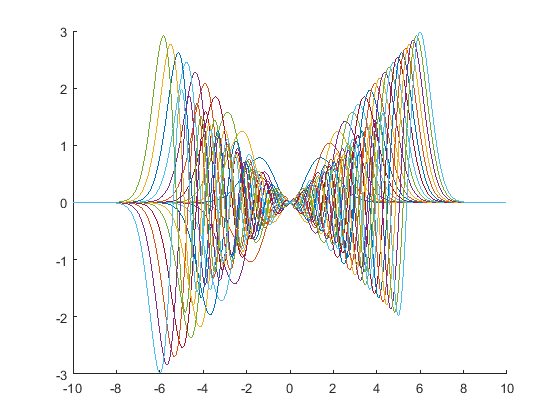
\includegraphics[width=\linewidth]{eigenstates.png}
  \caption{First 20 Eigen Function.}
  \label{fig:first 20 Eigen Function}
\end{figure}



\end{document} 